\subsection{Software Architektur}

Seit dem die ersten Großrechner gebaut wurden und ein Projekt nicht mehr von einem Team allein entwickelt werden konnte, entstand der Bedarf komplexe Systeme aufzuteilen und zu strukturieren. So war es schon in den 60er Jahren notwendig, die Entwicklung des  Betriebssystems OS/360 von IBM in mehrere Team aufzuteilen und klare Schnittstellen zwischen den Teilen zu bestimmen \parencite{brooks_mythical_1995}. Es entwickelte sich daraus eine der ersten Anwendungen und Umsetzungen von  Softwarearchitektur, welche erstmalig 1969 bei einer Softwaretechnik Konferenz in Rom auch als solche bezeichnet wurde \parencite[vgl.][S. 12]{buxton_software_1970}. In den darauf folgenden Jahren wuchs das Interesse an der Thematik und die Anwendungen der Teilung und Strukturierung von Softwaresystemen.
Hieraus entstand die im Jahr 2000 veröffentlichte Norm IEEE1471:2000, welche am 15. Juli 2007 als  ISO/IEC  42010 übertragen wurde. In diesem Standard werden Anforderungen an die Beschreibung von System-, Software- und Unternehmensarchitekturen definiert \parencite{hilliard_isoiecieee_nodate}.

\subsubsection{Definition}

%Todo Definition nach IEEE1471-2000 einfügen

Helmut Balzert, einer der führenden Pioniere im Bereich Softwarearchitektur und Autor der Bücherreihe \textit{Lehrbuch der Softwaretechnik}, beschreibt diese als \textit{\enquote{eine strukturierte oder hierarchische Anordnung der Systemkomponenten, sowie Beschreibung ihrer Beziehungen}} \parencite[][S. 580]{balzert_lehrbuch_2011}. Ihm nach lässt sich somit jedes System in mehrere einzelne Komponenten teilen, welche untereinander in Verbindung stehen und gemeinsam das Gesamtsystem formen.

Paul Clements, Autor der Bücher \textit{Software Architecture in Practice und Documenting Software Architectures: Views and Beyond}, schließt sich Balzert an und beschreibt Softwarearchitektur als \textit{\enquote{Strukturen eines Softwaresystems: Softwareteile, die Beziehungen zwischen diesen und die Eigenschaften der Softwareteile und ihrer Beziehungen}} \parencite[][S. 23]{clements_documenting_2010}.

Somit definieren beide Softwarearchitektur als Strukturierung von einzelnen Komponenten, die untereinander in Beziehung stehen. Dabei können sowohl die Komponenten als auch die Beziehungen Eigenschaften besitzen. Die einzelnen Komponenten zusammen ergeben das Gesamtsystem, welches in einer bestimmten Struktur vorliegt und beschrieben wird. Folglich beinhaltet die Softwarearchitektur alle nötigen Informationen über die Struktur der einzelnen Systemkomponenten und deren Kommunikationen untereinander.

%Todo Definition von Softwarearchitektur nach Martin Fowler einfügen und die relevanz von Entscheidungen auch Außerhalb von Technichen Entscheidungen (siehe Youtube Video).

%Todo Darauf eingehen, dass zum größten Teil auf die Technische Definition eingeganen wird.

Wird ein Softwaresystem in Komponenten geteilt, welches jedoch selbst eine Funktionalität besitzt, bedeutet dies, dass auch diese Logik in Teile geteilt wird und jede einzelne Komponente einen Teil erfüllt. Um gleichermaßen den selben Funktionsumfang, wie das Gesamtsystem bewältigen zu können, müssen die einzelnen Komponenten zusammenarbeiten. Demnach ist es wichtig, die Zuständigkeit jeder einzelnen Komponente genau zu klären und die Abhängigkeiten zu bestimmen. Auf Grund der Abhängigkeiten werden im Anschluss Schnittstellen definiert, über welche die einzelnen Komponenten Informationen austauschen können.

Bei der Teilung in einzelne Komponenten können bekannte Architekturstile helfen, da sich diese im Laufe der Zeit entwickelt haben und gut dokumentiert sind. Architekturstile sich dabei einige Regeln zur Strukturierung eines Systems und fassen Merkmale eines IT-Systems, sowohl hinsichtlich der Komponenten, als auch ihrer Kommunikation zusammen \parencite[vlg.][S. 102]{starke_effektive_2015}. Seit Beginn der Softwarearchitektur hat sich eine Vielzahl an solchen Stilen entwickelt, die aus unterschiedlichen Intention entstanden sind. Jedes System hat dabei unterschiedliche Herangehensweisen, sowie Vor- als auch Nachteile. Da die Lösung eines Problem von der eigentlichem Umsetzung unabhängig ist, können auch unterschiedliche Architekturstile zur ein und der selben Lösung verwendet werden. Hinsichtlich der Auswahl des Stiles gibt es demnach keine richtige oder falsche Antwort. Es ist viel mehr das Abwiegen von Pro und Kontra, sowie eine persönliche Präferenz der Entwickler.

Da die unterschiedlichen Architekturstile nicht im  Fokus dieser Bachelor Thesis sind, werden nur folgende Stile betrachtet:

\begin{enumerate}
	\item Verteilte Systeme,
	\item Interaktionsorientierte Systeme,
	\item REST-Architektur,
	\item Monolithe Architektur
\end{enumerate}

\subsubsection{Verteilte Systeme}

Nach Andrew Tanenbaum werden verteilte Systeme als eine Menge unabhängiger Computer bezeichnet, die dem Benutzer wie ein einzelnes, kohärentes System erscheinen \parencite{tanenbaum_verteilte_2007}. Weiterführend beschreibt Gernot Starke die einzelnen Komponenten als entweder Verarbeitungs-, oder Speicherbausteine, die über definierte Schnittstellen innerhalb eines Kommunikationsnetz zusammenarbeiten \parencite[vlg.][S. 116]{starke_effektive_2015}. Im Gegensatz zur Definition von Softwarearchitektur grenzt sich das verteile System dadurch ab, dass von unabhängigen Computer geredet wird. Dadurch entstehen einige Vorteile. So lassen sich auf Grund der Unabhängigkeit, diese einzelnen Rechner unterschiedlich skalieren. Es entsteht dadurch ein Netzwerk an heterogenen Computern. Somit kann je nach Anforderung der einzelnen Komponenten, eine entsprechende Rechenleistung genutzt werden. Des Weiteren gibt es auf Grund der Verteilung eine gewisse Ausfallsicherheit. Diese entsteht, da das Gesamtsystem nicht durch eine, sondern durch mehrere Maschinen getragen wird. Dadurch können einzelne Computer ausfallen ohne, dass das Anwendungssystem ausfällt. Jedoch kann dadurch ein Teil der gesamten Funktionalität wegfallen, der ggf. für das System notwendig ist. Um dies zu verhindern, sollten geeignete Maßnahmen getroffen werden, indem zum Beispiel nicht allein ein Computer für die Funktionalität verantwortlich ist, sondern mehrere.

Jedoch entsteht mit der Verteilung auch ein Anstieg der Komplexität, sowohl bei dem Konzipieren des Systems, als auch bei der Wartung und Managen dessen. Außerdem muss nicht nur ein Rechner abgesichert werden, sondern ein ganzes Netzwerk. Dadurch entsteht ein höherer Aufwand zur Absicherung.

Die einzelnen Computer können über verschiedene Mechaniken miteinander kommunizieren: Einerseits durch direkten Aufruf entfernter Funktionalität und andererseits durch indirekten Austausch von Informationen \parencite[vlg.][S. 116]{starke_effektive_2015}. Dabei kann der Transfer synchron oder asynchron ablaufen. Bei einem synchronen Aufruf, der nur direkt ausgelöst wird, führt ein Computer über das Netzwerk die Funktionalität eines anderen aus und wartet auf dessen Antwort \parencite{synchrone_2018}.
Bei einem asynchronen Aufruf wird entweder direkt oder indirekt Logik eines anderen Computer aufgerufen, während der aufrufende Rechner, ohne auf die Antwort zu warten, weiter verarbeitet. Ist die aufgerufene Rechner fertig gibt er das Resultat zurück, welches vom ersten Computer aufgenommen und verarbeitet wird \parencite{wiki_asynchrone_2019}.

%Todo Mit Müller klären ob Wikipedia als Quelle gilt.

Der Austausch von Informationen und das Aufrufen von externer Funktionalität kommt in einem System dauerhaft vor. Dadurch besteht das Risiko, dass einzelne Informationen verloren gehen können und das System sicherstellen muss, dass das Anwendungssystem nicht darunter leidet.

\subsubsection{Interaktionsorientierte Systeme}

Interaktionsorientierte Systeme zeichnen sich dadurch aus, dass sie den Fokus auf die Interaktion zwischen Mensch und Maschine legen \parencite[vgl.][S. 124]{starke_effektive_2015}.
Ein viel verwendeter Vertreter hiervon ist der Model-View-Controller Ansatz. Hierbei werden die einzelnen Komponenten in drei unterschiedliche Kategorien eingeteilt, von dem jeweils ein Repräsentant vorhanden sein muss. Eingeteilt wird in die drei Kategorien: Model, View und Controller, unterdessen jede Gattung eine eigene Funktion besitzt.

So kümmert sich das Model um die Datenspeicherung, den Datenabruf und Verarbeitung von Informationen und ist eine Verbindung zwischen dem Speichermedium und der Anwendung (siehe \cref{fig:mvc-cm-kommunikation} und \cref{fig:mvc-vm-kommunikation} Punkt 4 und 5 bzw. Punkt 5 und 6). Da jegliche Speicherung ausschließlich über das Model abläuft, wird dadurch das Speichern, sowie das Abrufen einheitlich geregelt.

Davon getrennt sind die graphischen Darstellungen, welche durch Views definiert werden. Sie erhalten ihre Informationen vom Model. Dabei können die Daten entweder direkt vom View angefordert (siehe \cref{fig:mvc-vm-kommunikation} Punkt 4) oder indirekt vom Controller übergeben werden (siehe \cref{fig:mvc-cm-kommunikation} Punkt 3 und 7). Unabhängig des Informationsflusses hilft es die Darstellung von der Restlichen Logik zu trennen, um eine einheitliche Verantwortung zu waren. Dies ist insbesondere empfehlenswert, da Dateien, zum beschreiben von Views, schnell unübersichtlich werden.

Der Controller hingegen kümmert sich, um die Verwaltung der Benutzereingabe und um das Aufrufen der Views (siehe \cref{fig:mvc-cm-kommunikation} und \cref{fig:mvc-vm-kommunikation} Punkt 2 und 7 bzw. Punkt 2 und 3). Er sorgt dafür, dass die Events oder Aktionen, die vom Benutzer über die Views auslöst werden, verarbeitet werden und führt entsprechende Datenverarbeitungen im Model aus. Falls notwendig lädt er auch Informationen aus der Datenbank und übergibt sie der entsprechenden View, welche er abschließend rendert.

Beim Model-View-Controller Ansatz handelt es sich um ein Muster, welches oft in der Softwarearchitektur verwendet wird, da es die Verantworlichkeiten trennt und das System somit verständlicher wird.
Im Unterschied zu verteilten Systemen stellt das Muster jedoch keine Anforderungen bezügliche der Hardware. Viel mehr beschreibt es eine Art den Quellcode hinsichtlich seiner Funktion zu teilen. Demnach kann dieser Stil auch für Codeteilung innerhalb einer Komponente verwendet werden und beschreibt nicht zwingend ein Architekturstil, der sich auf das Gesamtsystem besieht.

\begin{figure}
	\centering
	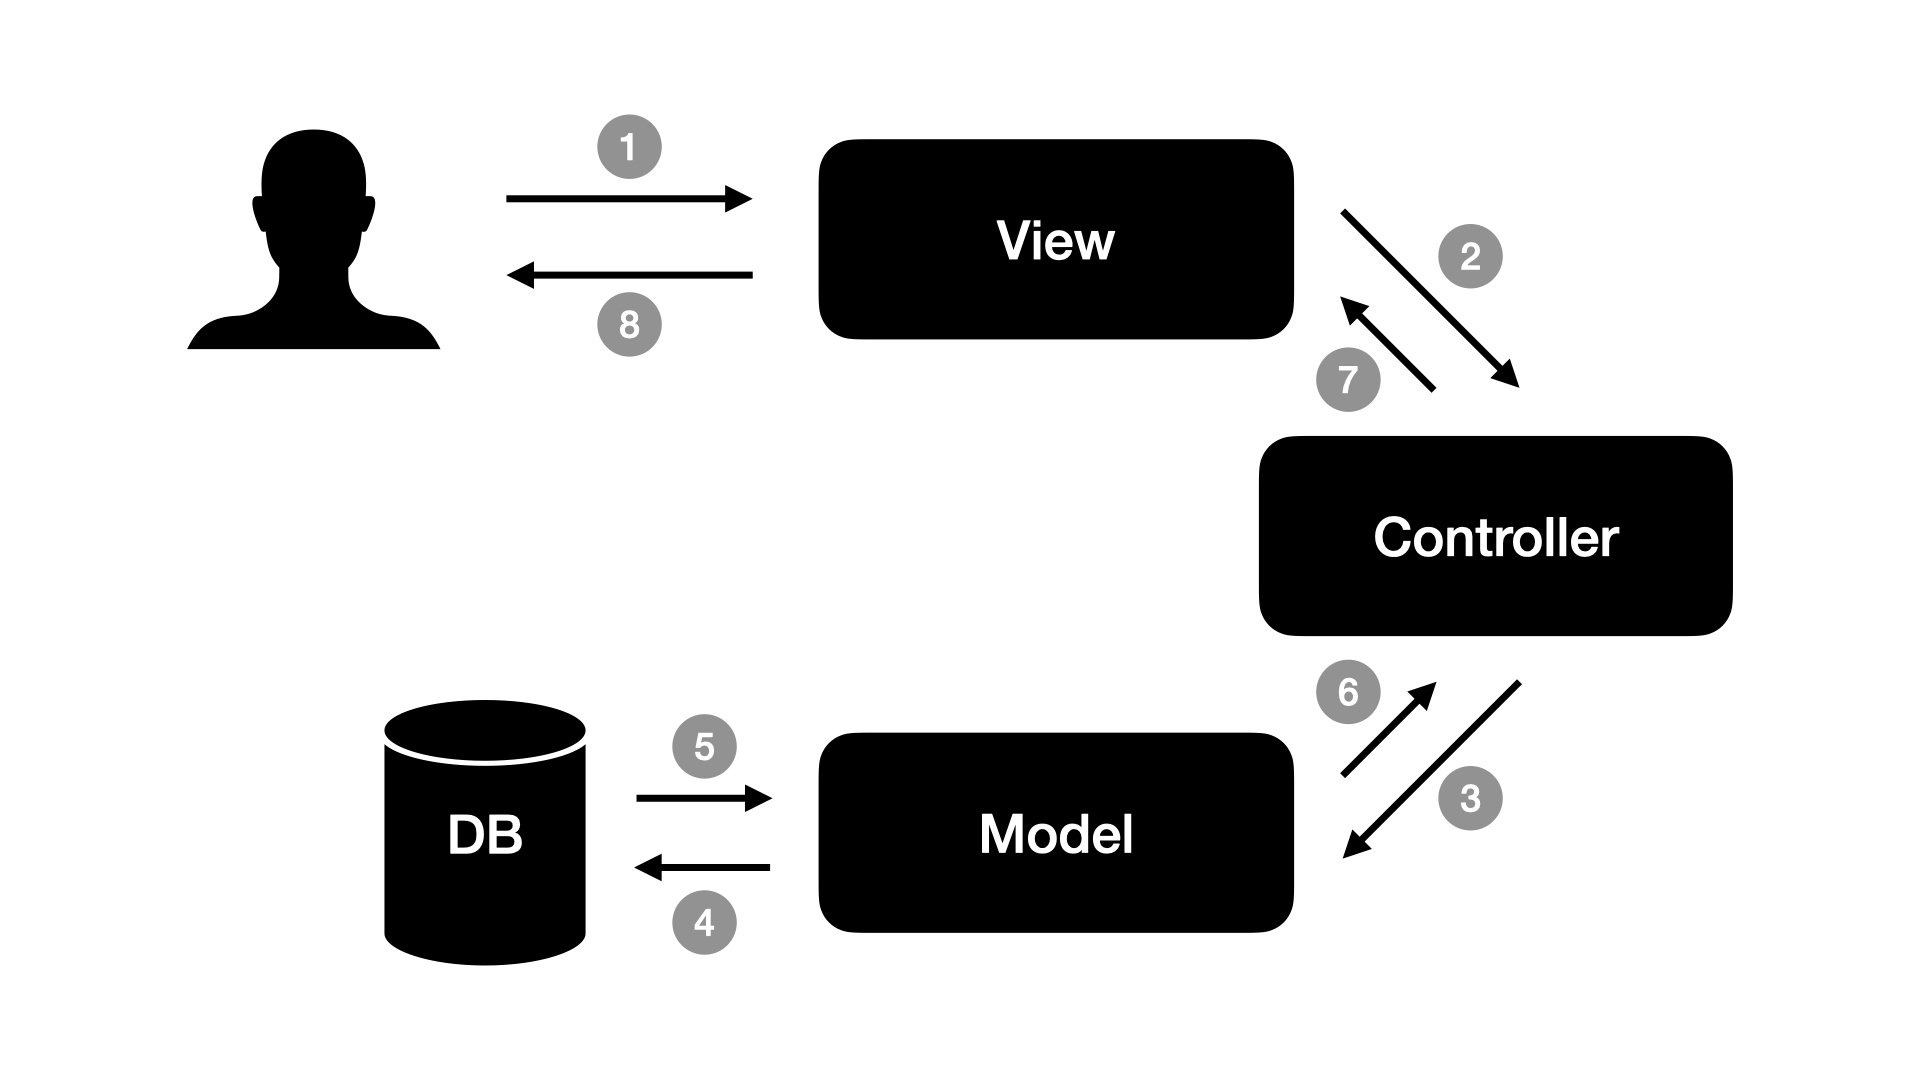
\includegraphics[width=.6\textwidth]{Assets/Interaktionsorientiert.001}
	\caption[Kommunikation zwischen Controller und Model]{Kommunikation zwischen Controller und Model, \\ (1) Der Benutzer sieht die graphische Darstellung und führt eine Aktion aus (2). Der Controller verarbeitet die Aktion und ruft über das Model Daten ab (3). Das Model greift auf die Datenbank zu und lädt die entsprechenden Informationen (4 und 5). Anschließend gibt es die Inhalte an den Controller zurück (6). Dieser gibt die Daten an die View weiter (7), welche Abschließend die neuen Inhalte dem Benutzer anzeigt (8).}
	\label{fig:mvc-cm-kommunikation}
 \end{figure}
 
 \begin{figure}
 	\centering
    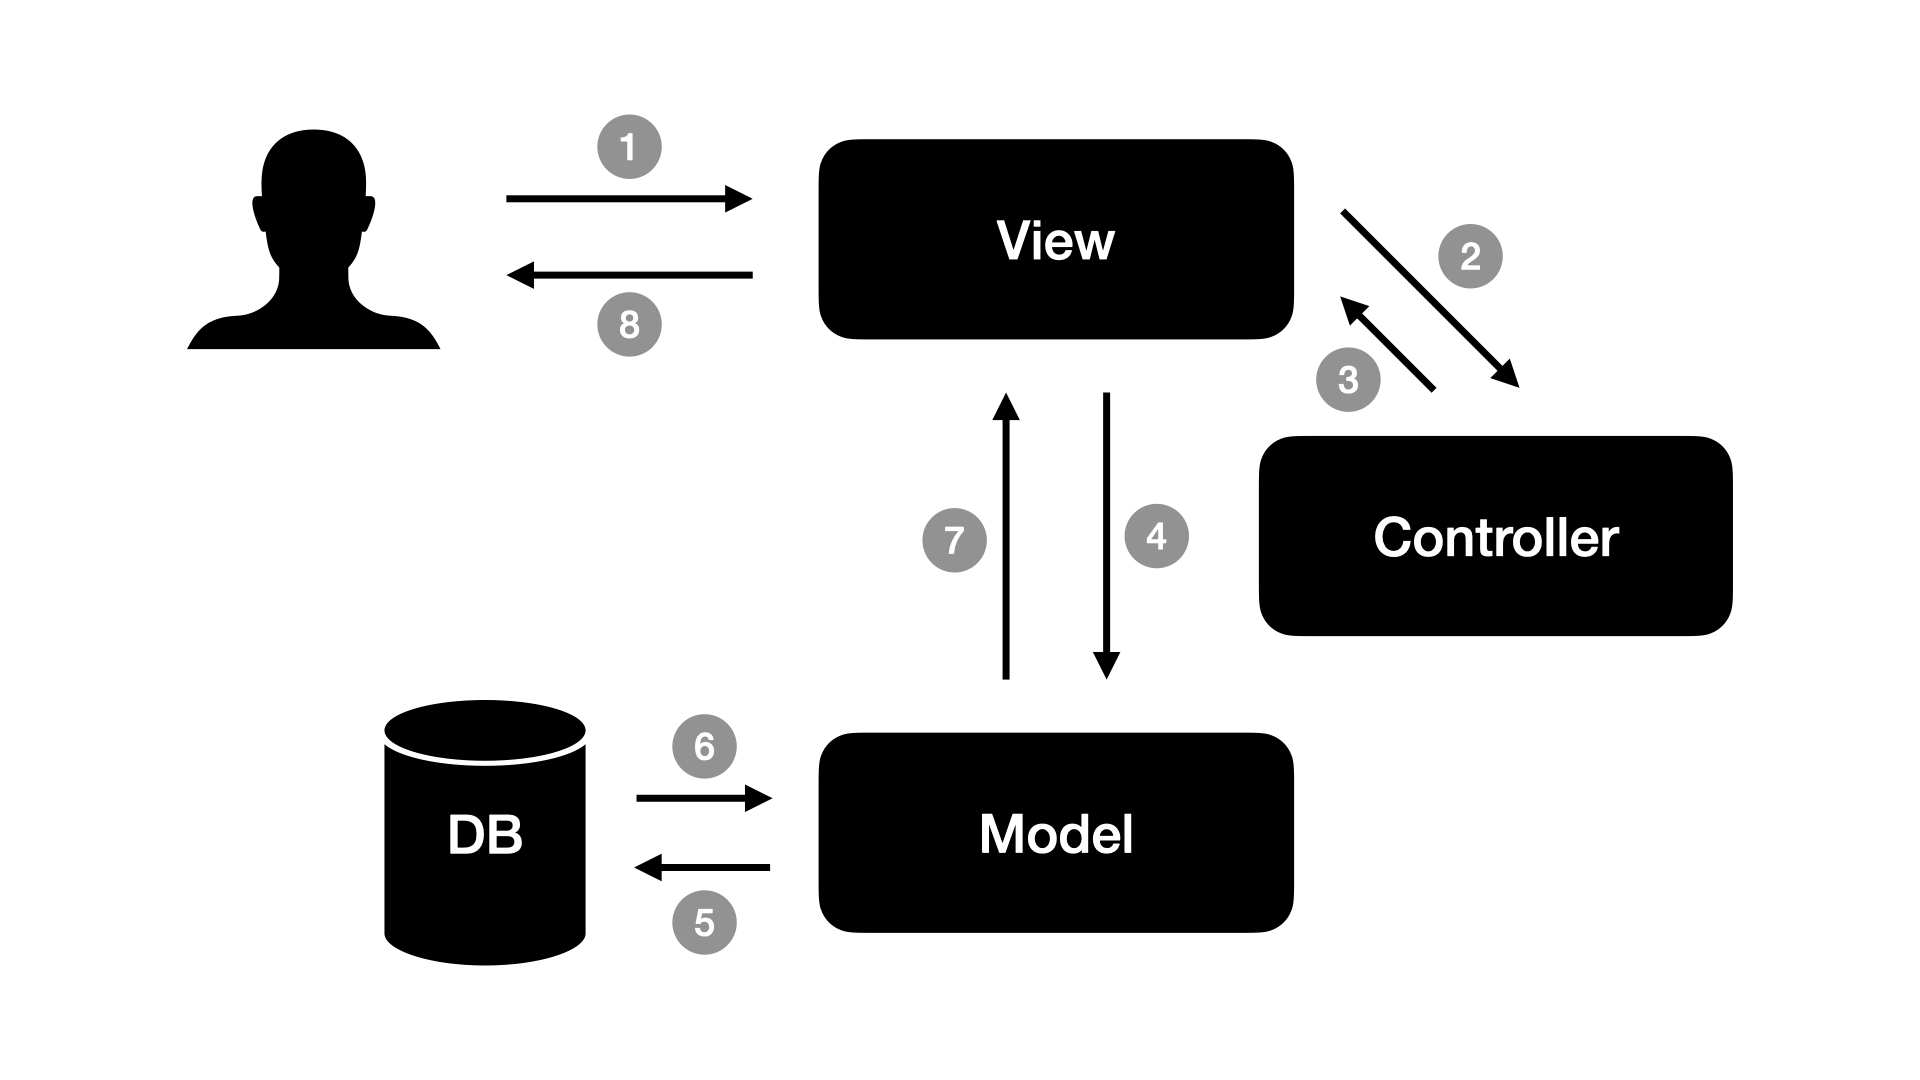
\includegraphics[width=.6\textwidth]{Assets/Interaktionsorientiert.002}
	\caption[Kommunikation zwischen View und Model]{Kommunikation zwischen View und Model, \\ (1) Der Benutzer sieht die graphische Darstellung und führt eine Aktion aus (2). Der Controller verarbeitet die Aktion und rendert umgehend die graphische Darstellung (3). Der View lädt über das Model die Daten (4). Das Model greift auf die Datenbank zu und lädt die angeforderten Informationen (5 und 6). Anschließend gibt es die Inhalte an den View zurück (7). Dieses Abschließend die neuen Inhalte dem Benutzer anzeigt (8).}
    \label{fig:mvc-vm-kommunikation}
 \end{figure}

\subsubsection{REST-Architektur}

Neben den bislang genannten Architekturstilen gibt es eine Vielzahl von weiteren Strukturierungen, die sich erst in den letzten 20 Jahre entwickelt haben. Einer dieser Architekturstile ist die REST-Architektur, welche vom Miterfinder des HTTP-Standards Roy Fielding definiert wurde \parencite[][S. 128]{starke_effektive_2015}. Er beschrieb diesen Stil in seiner Dissertation an der Universität von Kalifornien im Jahr 2000 und charakterisiert ihn als Architekturstil fürs Web.

Dabei steht REST für \textit{Representationl State Transfer}, welches ein Architekturstil für verteilte Systeme beschreibt und auf der Server-Client Architektur aufbaut \parencite[][S. 76]{fielding_architectural_2000}. Server-Client Architektur beschreibt eine Ausprägung eines verteilten Systems, bei dem die Anwendung in Server und Clients geteilt werden \parencite[][S. 117]{starke_effektive_2015}.\footnote{Dabei beziehen sich die Begriffe \textit{\enquote{Server}} und \textit{\enquote{Client}} auf software Komponenten und auf den physischen Server und das Endgerät des Nutzers (Client). Des Weitern grenzt sich der  Architekturstil von der Mainframe Architektur ab, bei der über Terminals Anweisungen an ein Großrechner gestellt werden.}

Ein Server ist dabei eine software Komponente im Netzwerk, welches Services anbietet. Ein Service könnte zuständig sein, alle Informationen der hinterlegten Kunden auszugeben. Der Client hingegen konsumiert lediglich diese Informationen und dient dem Benutzer als Bedienungsoberfläche. Dies bedeutet, dass der Server nur passiv auf Anfragen vom Client wartet, während der Client selbst keine Informationen verarbeitet, sondern ausschließlich anzeigt. Nichtsdestoweniger handelt es sich um ein Programm, welches auf dem Endgerät des Benutzers (Computer, Mobiltelefon) ausgeführt wird.

Die REST-Architektur verwendet diese Aufteilung, um eine feste Trennung der Zuständigkeit zu integrieren \parencite[vgl.][S. 78]{fielding_architectural_2000}.

Die zweite Bedingung, die Fielding an den Architekturstil gestellt hat, ist dass die Kommunikation zustandslos, zu englisch (stateless), abläuft \parencite[][S. 78]{fielding_architectural_2000}. Dies bedeutet, dass die Nachrichten, die zwischen Server und Client ausgetauscht werden, alle nötigen Informationen beinhalten \parencite[][S. 128]{starke_effektive_2015}. Somit gibt der Server auf Anfrage des Clients stets die gleiche Antwort zurück, egal ob dieser zum ersten, oder wiederholten Mal angefragt wurde. Des Weiteren hängt die Antwort nicht vom Client ab.
Diese Entkopplung zwischen den Komponenten ermöglicht, dass die Aufgabe des Server, sowie des Clients durch mehrere Computer verrichtet werden kann und somit das System skalierbar ist \parencite[][S. 79]{fielding_architectural_2000}.

Der Hauptunterschied zwischen der REST-Architektur und anderen Stilen liegt jedoch in der genauen Bestimmung der zu verwendeten Kommunikationsschnittstellen. So bestimmt die REST-Architektur sehr explizit, welche From zur Kommunikation verwendet werden darf. Anders als andere Stile beruht der Aufruf von Methodiken nicht auf individuelle Funktionalität, sondern auf dem HTTP-Standard. Konkret bedeutet dies, dass die einzelnen Dienste des Servers sich an die HTTP-Optionen (GET, PUT, POST und DELETE) richten und keinen eigenen verwenden \parencite[vlg.][S. 128]{starke_effektive_2015}. Somit baut die REST-Architektur auf ein Kommunikationsstandard auf, der sich im Internet etabliert hat.

Auf Grundlade der standardisierten Kommunikation können zwischen Server und Client intelligente Zwischenstationen geschalten werden, die dazu zuständig sind häufig vorkommende Anfragen abzuspeichern \parencites[vlg.][S. 79 f.]{fielding_architectural_2000}[][S. 128]{starke_effektive_2015}. Somit lässt sich eine Vielzahl von Serveranfragen im vornherein beantworten.

Die Antwort des Servers erfolgt durch Repräsentationen der Daten, wovon es für jede Ressource mehr Formate gibt. So kann eine Schnittstelle abhängig des angeforderten Mediums, sowohl JSON­, als auch XML­ oder HTML zurück geben \parencite[vgl.][S. 128]{starke_effektive_2015}.

Verwendet wird die REST-Architektur ausschließlich für Anwendungen im Internet, da es auf die Anwendung des Hypertext Transfer Protokoll\footnote{Weitere Informationen zum Hypertext Transfer Protokoll kann unter folgender Literatur gefunden werden \parencite{leach_hypertext_2020}.} (HTTP) angewiesen ist. Dabei findet der Architekturstil, sowohl Anwendung für ganze Systeme, als auch in komplexen Anwendungen mit einer Vielzahl ein einzelnen Services.

%Todo Korrekturlesen von Yola

\subsubsection{Monolithe Architektur}

Der Begriff \textit{\enquote{Monolith}} leitet sich vom altgriechischen \textit{\enquote{monólithos}} ab und bedeutet \textit{\enquote{aus einem Stein}} \parencites[vlg.][]{duden_nodate}[vgl.][]{dwds_nodate}. In der Gesteinskunde wird damit ein natürlich entstandener Gesteinsblock bezeichnet, der komplett aus einer Gesteinsart besteht \parencite[vgl.][]{dwds_nodate}.

Nach Rod Stephens liegt eine monolithische Softwarearchitektur vor, wenn jegliche Funktionalität des Systems miteinander verbunden ist. Dabei spricht er auf die Verbindung von Dateneingabe, Datenausgabe, Datenverarbeitung, sowie Fehlerhandhabung und Benutzeroberflächen \parencite[vgl.][S. 94]{stephens_beginning_2015}.

Anders sieht es Sam Newman. Ihm nach liegt ein Monolites System schon vor, wenn die gesamte Funktionalität eines Systems gemeinsam über ein Deployment-Prozess bereitgestellt wird \parencite[vgl.][Kap. 2.2]{newman_monolith_2019}. Somit muss nicht zwingend jegliche Logik miteinander verbunden sein. Er unterteilt Monolithe Systeme in drei Kategorien: Einzelprozess Monolithe, Modulare Monolithe und verteilte Monolithe \parencite[vgl.][Kap. 2.2]{newman_monolith_2019}.

Der Einzelprozess Monolith ist die gängigste Form und deckt sich mit der Definition von Rod Stephens. Somit handelt es sich dabei, um ein System bei dem das gesamte System ein Prozess abbildet. Dies bedeutet, dass jegliche Funktionalität auf einander aufbauend ist und nur eine Datenspeicherung für die gesamte Anwendung verwendet wird \parencite[vgl.][Kap. 2.2.1]{newman_monolith_2019}.

Anders ist dies beim Modularen System. Dieses zeichnet sich darin aus, dass die Funktionalität in einzelne Module geteilt wird und sogar einzelne Module eine separate Datenspeicherung besitzen können \parencite[vgl.][Kap. 2.2.2]{newman_monolith_2019}. Diese Form von monolithen System ist jedoch seltener und wird nur von einzelnen Unternehmen eingesetzt.

Im Gegensatz zu verteilten Systemen sind die einzelnen Komponenten nicht auf separaten Computern verteilt und werden durch einen Deployment-Prozess online gestellt. Des Weiteren sind die einzelnen Module nur leicht entkoppelt, so kann es immer noch Abhängigkeiten geben \parencite[vgl.][Kap. 2.2.2]{newman_monolith_2019}. Unterschiedlich davon sind verteilte Monolithe. Diese sind komplett entkoppelt und kommunizieren nur noch über definierte Schnittstellen \parencite[vlg.][S. 116]{starke_effektive_2015}. Sie erfüllen somit jegliche Anforderungen an ein verteiltes System, sind jedoch in einem einzigen Bereitstellungsprozess gebündelt. Diese From wird jedoch kaum verwendet.

Weder Stephens, als auch Newman geben Vorgaben hinsichtlich der Gliederung innerhalb eines Monolithischen Systems. Demnach kann eine Model-View-Controller Ansatz als Monolithisches System gelten, solange es einheitlich deployed wird. Anders ist es mit einem verteilten System, da nach Definition ein Monolithen System kein verteiltes System sein kann. 

Im Rahmen dieser Arbeit wird bei jeglichen weiteren Referieren auf den Begriff Monolithen System stets von einem Einzelprozess Monolithen ausgegangen, außer es wird expliziert von einem Modularen, oder verteilten Monolithen geschrieben. Dadurch sollen beide Definitionen berücksichtig werden.

Im Vergleich zu einem verteilten System gibt es einige Vor- als auch Nachteile \parencite[vgl.][Kap. 2.2.4 und Kap. 2.2.5]{newman_monolith_2019}. So ist das bereitstellen eines Monolithen System einfacher, da es ein Bereitstellungsprozess für die gesamte Anwendung gibt. Wiederum führt dies dazu, dass der Prozess deutlich länger dauert. Diese Tatsache ist insbesondere gravierend, wenn vermehrt kleine Änderungen vorgenommen werden. Anderseits vereinfacht eine Anwendung, die als ein Prozess zu sehen ist, die Fehlersuche und ermöglicht es Funktionen mehrfach zu verwenden. So lassen sich Funktionen und Klassen in einem Einzelprozess Monolithen mehrfach verwenden und schneller neue Funktionen umsetzen. Jedoch verursacht dies, dass schnell Abhängigkeiten entstehen können und Änderungen ungewollte Fehler verursachen. Dadurch wird die Umsetzung von neuen Funktionen mit steigender Codemenge verlangsamt und der Einstieg von neuen Teammitgliedern erschwert.

Bei größeren Unternehmen mit mehreren Team kommt hinzu, dass es leicht zu Konflikten kommen kann, da alle auf die gleiche Codebase zugreifen. So führt ein Monolithen System dazu, dass bei vielen Entwickler viele Absprachen nötig sind und es zu Problemen bei der Zusammenführung von Funktionen kommen kann \parencite[vgl.][Kap. 2.2.4]{newman_monolith_2019}. Anders ist es beim Erstellen von System übergreifenden Test. Diese werden durch ein Monolithen System begünstigt und können im Vergleich zu einem verteilten System einfacher umgesetzt werden  \parencite[vgl.][Kap. 2.2.5]{newman_monolith_2019}.

\subsubsection{Einordnung des aktuellen Systems von PluraPolit}

Wie aus der Einleitung hervorgeht, bietet PluraPolit eine Plattform an, die Jung- und Erstwähler bei der politischen Bildung hilft. Dafür wurde ein Softwaresystem entwickelt, in welches sich zum einen leicht neuer Content einpflegen lässt und zum anderen die hinterlegten Tonaufnahmen den Benutzern darstellt. Um diese zu erreichen wurde neben der eigentlichen Plattform eine Content Management System (CMS) konzipiert. Umgesetzt wurde dies in einer Ruby on Rails Anwendung mit Zugriffsbeschränkung durch Passwortabfrage.

Ruby on Rails, kurz auch Rails bezeichnet, ist ein quellenoffenes Webframework, welches für die Programmiersprache Ruby entwickelt wurde \parencites[vgl.][S.4]{hartl_ruby_2016}{ruby_org}[vgl.][S. 24]{sieben_wochen}. Es ist komplett Open Source und wird von einer aktiven Community entwickelt. Es gibt eine Vielzahl von kostenfreien Paketen, sogenannte Gems, die bei Belieben zu einem Projekt hinzugefügt werden können. Im Vergleich zu anderen Frameworks zeichnet sich Rails besonders durch seine Implementierung der REST-Architektur aus \parencite[vgl.][S. 5]{hartl_ruby_2016}. Diese Implementierung führt jedoch dazu, dass eine Vielzahl an Bedingungen an die Entwicklung und Implementierung von Rails Anwendungen gestellt werden. Getreu dem Motto \textit{\enquote{Konvention vor Konfiguration}} nutzt Rails die Bestimmungen als Vorteil und integriert ein System, indem externe Pakete ohne Konfigurationsaufwand hinzugefügt werden können \parencite{ruby_doctrine}.

% Todo noch einmal überarbeiten
Dabei orientiert sich Rails bei der Teilung der Dateien an dem Model-View-Controller-Ansatz \parencites[vgl.][S. 66 ff.]{hartl_ruby_2016}.

\begin{figure}
	\centering
	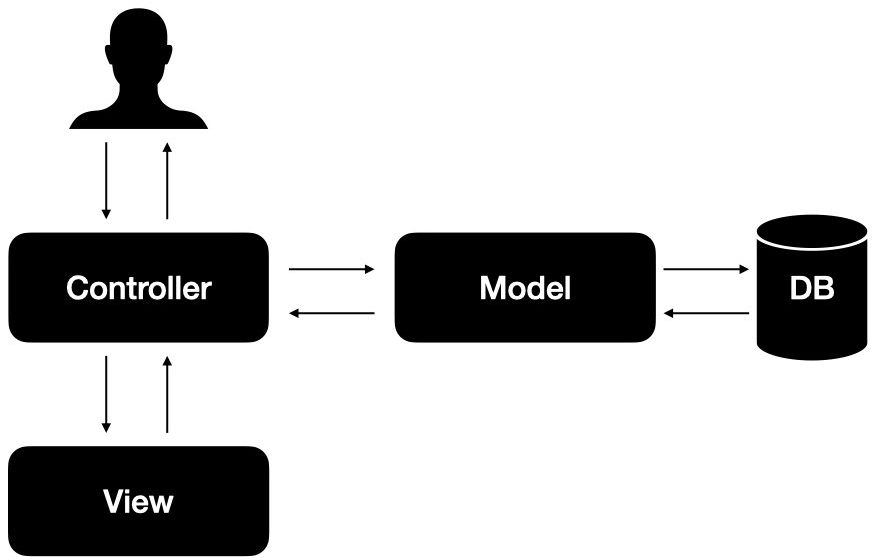
\includegraphics[width=0.6\textwidth]{Assets/CMS_V1}
	\caption{Darstellung des Model-View-Controller-Ansatz}
	\label{fig:mvc-plurapolit}
\end{figure}

% Todo Der Erste Satz ist noch etwas komplex und sollte ein zwei Teile gepackt werden.
% Um eine neue Tonaufnahme einzupflegen muss eine Url aufgerufen werden. Controller kommt in Aktion.
 Für das Einpflegen von neuen Tonaufnahmen bedeutet dies konkret, dass anhand der Eingabe der Url der für das verwalten von Tonaufnahmen zuständige Controller die gewünschte Darstellung anzeigt.
Darauf hin kann die Aufnahme als Datei hochgeladen werden. Dies geschieht, indem per Klick im CMS ein HTTP-Anfrage mit der geladenen Datei an den Controller geschickt wird. Dieser kümmert sich anschließend darum, dass die Datei über das Model in der Datenbank gespeichert wird und gibt die Bestätigung der Aktion im View wieder (siehe \cref{fig:mvc-plurapolit}).

Dabei wird die Tondatei selbst nicht in der Datenbank gespeichert. Vielmehr wird der Speicherservice von Amazon Web Services (S3) genutzt. Somit sendet, nachdem die Datei im View hinterlegt wurde, der Controller die Datei automatisch an S3 und erhält anschließend eine Url zurück. Diese wird anschließend abgespeichert und dient als Referenz zur eigentlichen Tonaufnahme (siehe Abbildung).

Neben dem Hochladen von Tonaufnahmen dient jedoch das CMS auch dazu bestehende Informationen zu bearbeiten und ggf. anzupassen.
% Todo Worauf bezieht sich das Detail - genauer beschreiben worauf sich das "Im Detail" bezieht.
% Aufruf der Webseite zum bearbeiten.
Im Detail bedeutet dies, dass die jeweilige Webseite per Url Aufruf angefragt wird, der Controller die angeforderten Daten über das Model aus der Datenbank lädt und die Entsprechende graphische Darstellung rendert. Dabei übergibt der Controller die Informationen an den View, der anschließend die Daten über Embedded RuBy in HTML integriert und anzeigt (siehe Abbildung).

% Todo Warum ist der Workflow für den user wichtig. Es ist noch nicht klar, dass der User die Daten bearbeiten möchte.

Auch die Plattform ist in Ruby on Rails implementiert. Genauer beschrieben handelt es sich bei der Plattform um die selbe Applikation wie das CMS nur das die graphische Darstellung durch das JavaScript Framework React übernommen wird. Im Detail bedeutet dies, dass beim Aufruf der Plattform eine Anfrage an den Controller geschickt wird und dieser anschließend die kompilierte React Anwendung ausgibt. Diese lädt eigenständig jegliche Informationen über HTTP Anfragen und kümmert sich um interne Seitenaufrufe. Die Anfragen werden dabei asynchron an die Rails Applikation geschickt und vom Controller beantwortet. Somit erhält die React Anwendung über die Kommunikation von Controller und Modul, den Content aus der Datenbank, der vorher eingepflegt wurde (Siehe Abbildung).

Demnach gibt es eine Aufteilung hinsichtlich der graphischen Darstellung in Content Management System und Plattform. Die Datenspeicherung und Verwaltung ist jedoch gleich. Auch wird die gesamte Codebase in einem Bereitstellungsprozesses dem Hosting Service bereit gestellt. Somit handelt es sich beim System von PluraPolit um ein Monolith, welches teilweise Modular ist, die REST-Standards erfüllt und nach dem Model-View-Controller-Ansatz aufgeteilt ist. Des Weiteren nutz es vereinzelt externe Services von AWS, um Tondateien zu speichern und Transcripierungen vorzunehmen.

%Todo Bilder erstellen und einfügen 
% Todo anderen Namen für Plattform, Nutzersicht, User-Plattform, PluraPolit-Webseite